%%%%%%%%%%%%%%%%%%%%%%%%%%%%%%%%%%%%%%%%%%%%%%
%                insertmeeting
% 1) Title (something creative & funny?)
% 2) Date (MM/DD/YYYY)
% 3) Location (ex. Hagerty High School)
% 4) People/Committees Present 
% 5) Picture 
% 6) Start Time & Stop Time (ex. 12:30AM to 4:30PM)
%%%%%%%%%%%%%%%%%%%%%%%%%%%%%%%%%%%%%%%%%%%%%%
\insertmeeting 
	{Cool Carbon} 
	{02/23/22} 
	{Hagerty High School}
	{James, Jensen, Samantha, Anouska, Annika, Clayton, Falon, Nathan, Ritam}
	{Images/RobotPics/robot.jpg}
	{2:30 - 4:30}
	
\hhscommittee{Hardware}
\noindent\hfil\rule{\textwidth}{.4pt}\hfil
\subsubsection*{Goals}
\begin{itemize}
    \item Manage the wires to ensure easy access and place the Spinner on the robot

\end{itemize} 

\noindent\hfil\rule{\textwidth}{.4pt}\hfil

\subsubsection*{Accomplishments}
Today, Mr. Harper taught me how to properly cable manage the wires of the robot. The first step was ensuring that all of the wires were plugged in properly. We did this by checking connections through a list that Ritam made. After checking connections, we began to move the wires to where they needed to be and make sure tension was just right. Then we put the wires through the pockets at the base of the drivetrain. This let us ensure that the wires for the drivetrain wouldn't get in the way. Then we Zip-tied the wires to ensure they would not spread out. Though Velcro is reusable, in our experience small sized zip ties are more compact and allow for better cable management. After that, we reattached the Carbon Fiber sides in order to protect the inside of the robot and make sure that the arm is fully supported. After this, we realized that, though we plugged in the spinner, it was not mounted in the way we like. To fix this we took the spinner off and used the belt sander to ensure that the spinner does not go against the carbon fiber. Though the placement is good, there is concern over the screws and tilting of the spinner. When the robot drives into the carousel, there is pressure put against the spinner. Because of the placement of the screws, it is weaker and will face more force against it. We may need to change that if it becomes a problem.

\begin{figure}[htp]
\centering
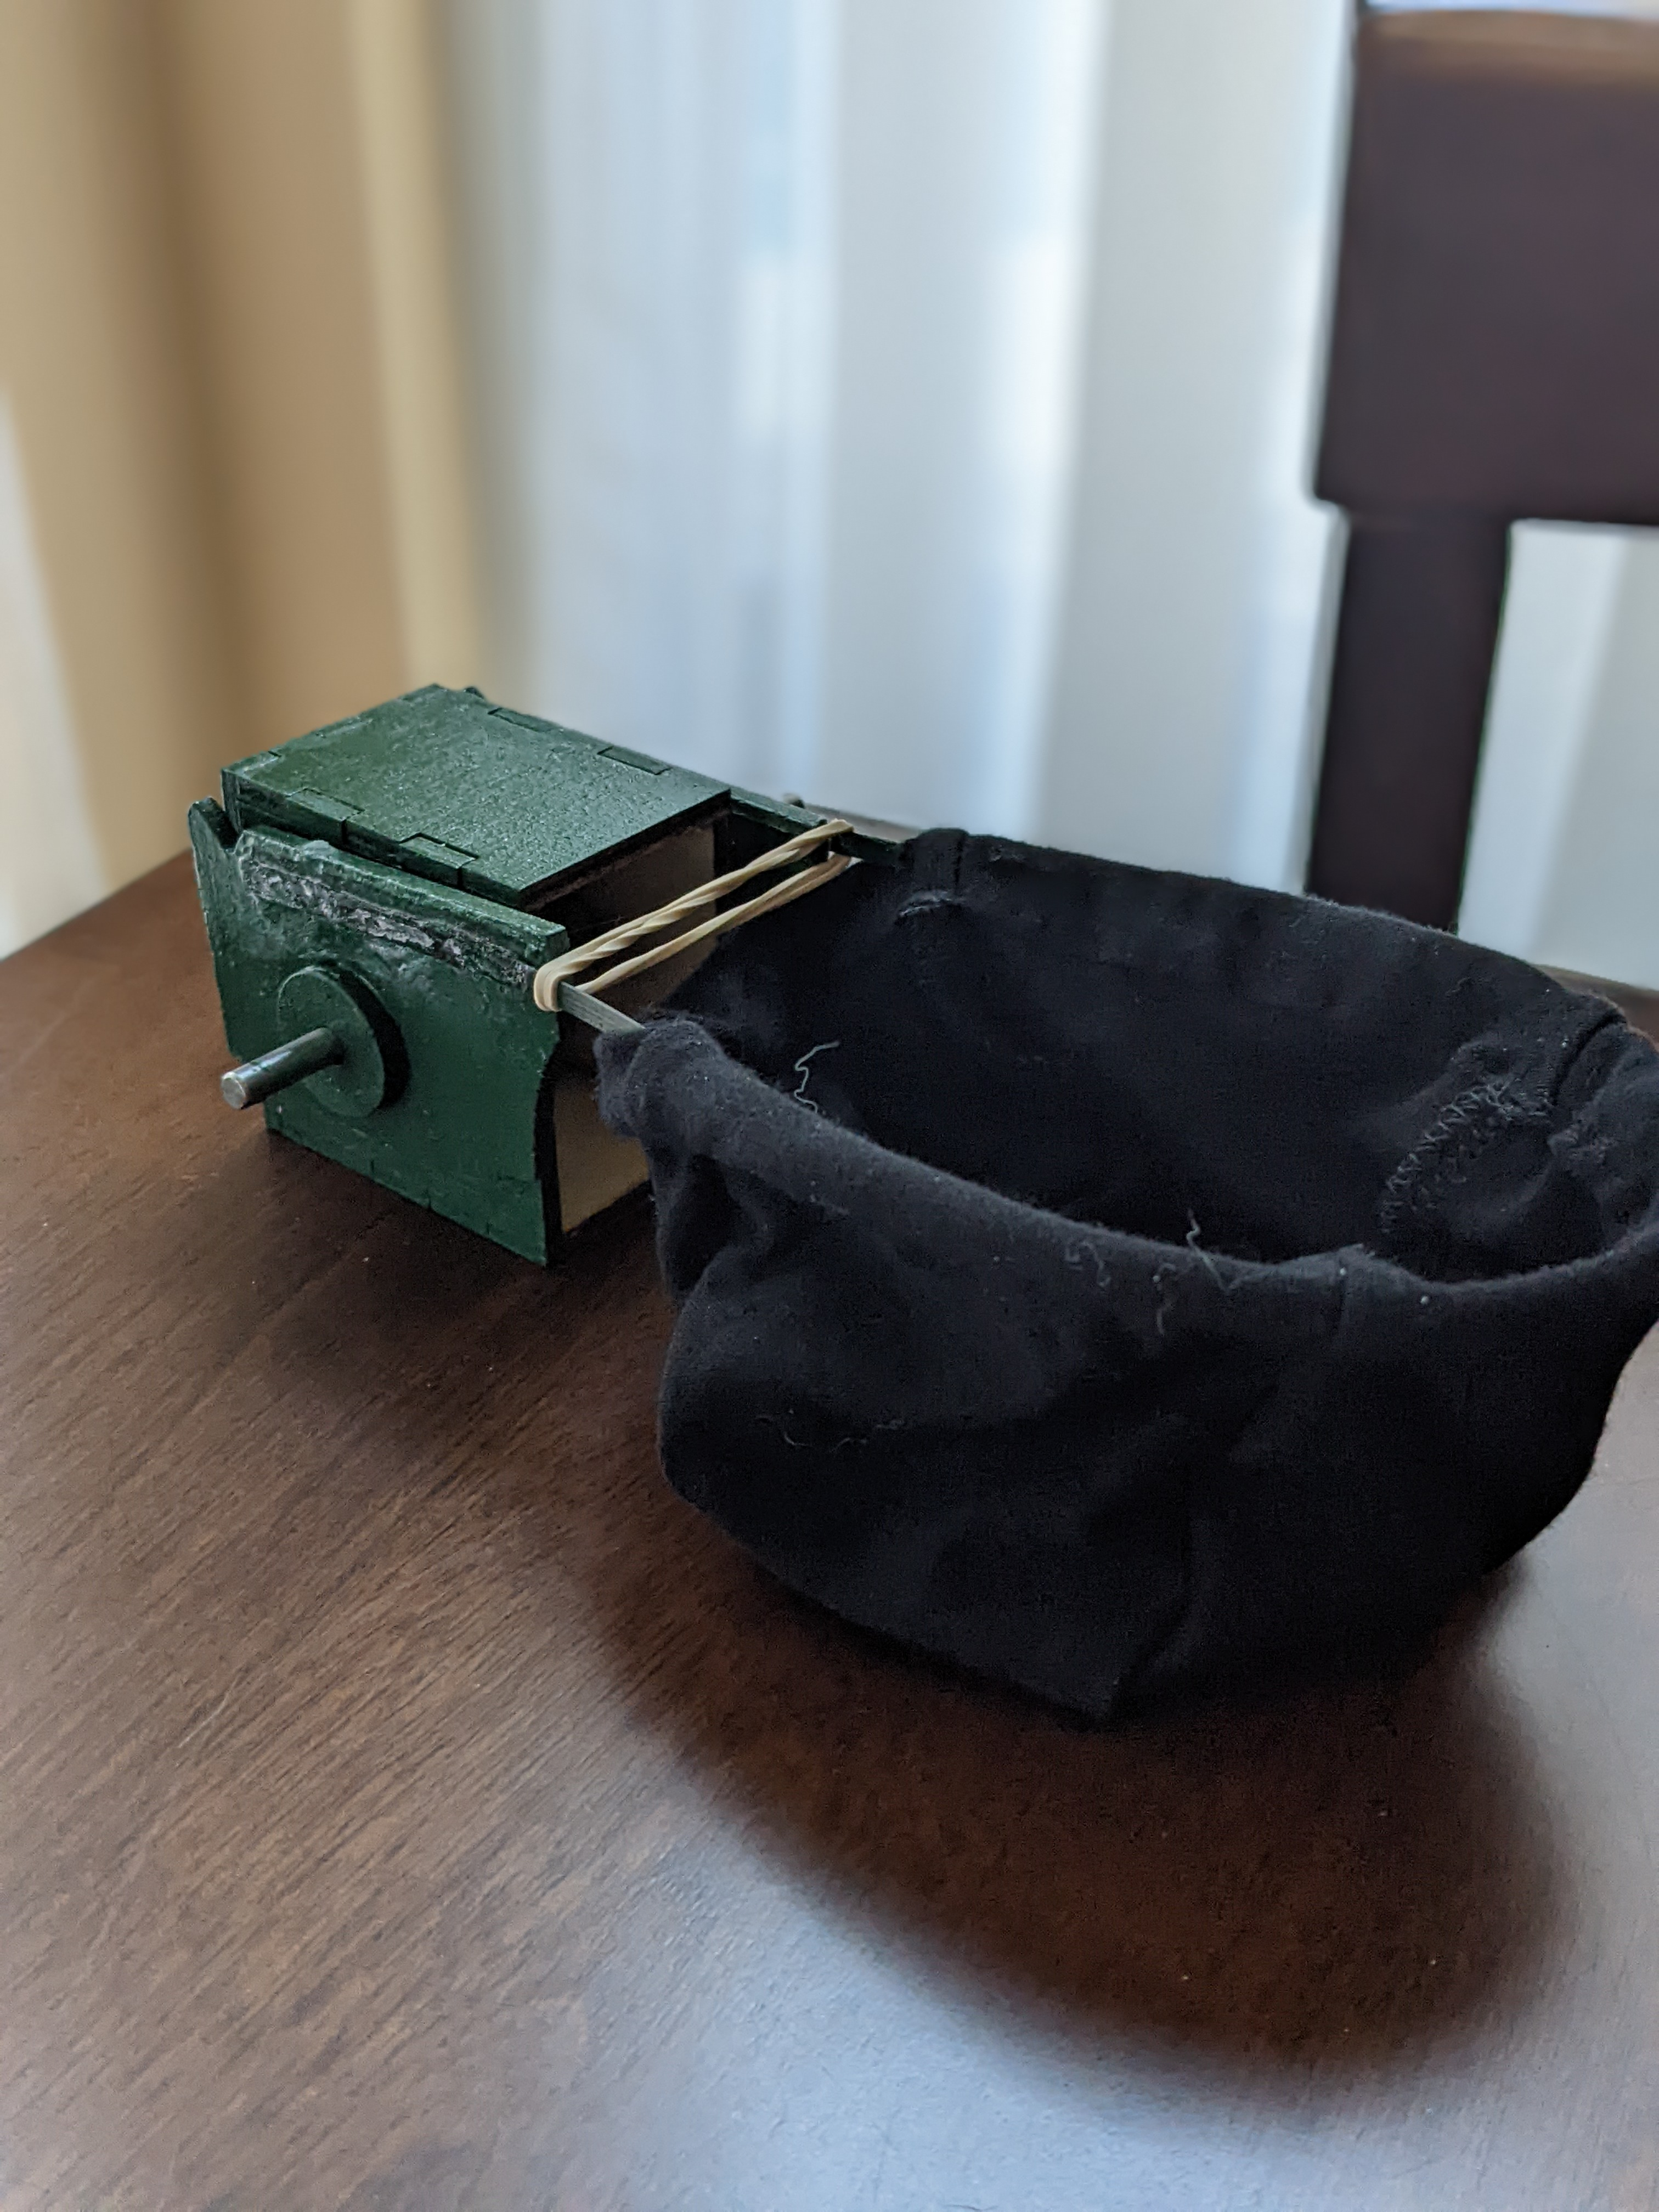
\includegraphics[width=0.95\textwidth, angle=0]{Meetings/February/02-23-22/02-23-22 1.jpg}
\caption{Our new capstone}
\label{fig:022322_1}
\end{figure}


\whatsnext{
\begin{itemize}
    \item 3D print the Element

\end{itemize} 
}

